% --------------------------------------------------------------
% This is all preamble stuff that you don't have to worry about.
% Head down to where it says "Start here"
% --------------------------------------------------------------
 
\documentclass[12pt]{article}

\usepackage[margin=1in]{geometry} 
\usepackage{amsmath,amsthm,amssymb}
\usepackage[margin=1in]{geometry} 
\usepackage{amsmath,amsthm,amssymb}
%\usepackage[spanish]{babel} %Castellanización
\usepackage[T1]{fontenc} %escribe lo del teclado
\usepackage{inputenc} %Reconoce algunos símbolos
\usepackage{lmodern} %optimiza algunas fuentes
\usepackage{graphicx}
\graphicspath{ {images/} }
\usepackage{hyperref} % Uso de links

% To Display Chinese words
\usepackage{xeCJK}
% To Display Code
% \usepackage{listings}
\usepackage{minted}
% To Display csv file
\usepackage{csvsimple}
\usepackage{longtable}
\usepackage{booktabs}
 
\newcommand{\N}{\mathbb{N}}
\newcommand{\Z}{\mathbb{Z}}
 
\newenvironment{theorem}[2][Theorem]{\begin{trivlist}
\item[\hskip \labelsep {\bfseries #1}\hskip \labelsep {\bfseries #2.}]}{\end{trivlist}}
\newenvironment{lemma}[2][Lemma]{\begin{trivlist}
\item[\hskip \labelsep {\bfseries #1}\hskip \labelsep {\bfseries #2.}]}{\end{trivlist}}
\newenvironment{exercise}[2][Exercise]{\begin{trivlist}
\item[\hskip \labelsep {\bfseries #1}\hskip \labelsep {\bfseries #2.}]}{\end{trivlist}}
\newenvironment{problem}[2][Problem]{\begin{trivlist}
\item[\hskip \labelsep {\bfseries #1}\hskip \labelsep {\bfseries #2.}]}{\end{trivlist}}
\newenvironment{question}[2][Question]{\begin{trivlist}
\item[\hskip \labelsep {\bfseries #1}\hskip \labelsep {\bfseries #2.}]}{\end{trivlist}}
\newenvironment{corollary}[2][Corollary]{\begin{trivlist}
\item[\hskip \labelsep {\bfseries #1}\hskip \labelsep {\bfseries #2.}]}{\end{trivlist}}

\newenvironment{solution}{\begin{proof}[Solution]}{\end{proof}}

% write csv content in latex 
\begin{filecontents*}{dqn.csv}
mean, max, min, median, count, max step
200, 200, 200, 200, 100, 200
\end{filecontents*}

\begin{filecontents*}{ddpg.csv}
mean, max, min, median, count, max step
-153.861, -2.256, -533.589, -123.861, 1000, 100
\end{filecontents*}
 
\begin{document}
 
% --------------------------------------------------------------
%                         Start here
% --------------------------------------------------------------
 
\title{2019 Deep Learning and Practice \\ Lab 8 -- Deep Q-Learning and Deep Deterministic Policy Gradient}
\author{0756110 李東霖}

\maketitle
\section{DQN's episode rewards in training}

\begin{figure}[H]
\centering
% \includegraphics[width=\linewidth]{path/to/image}
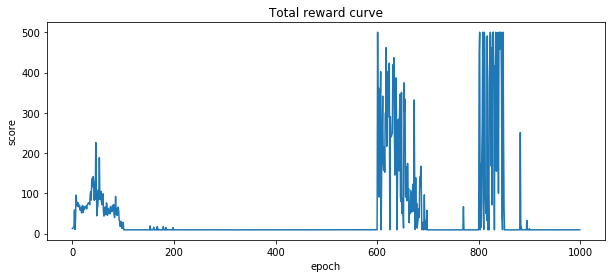
\includegraphics[width=\linewidth]{Images/dqn-rewards.png}
\caption{DQN average of total reward in 100 testing}
\end{figure}

\section{DDPG's episode rewards in training}

\begin{figure}[H]
\centering
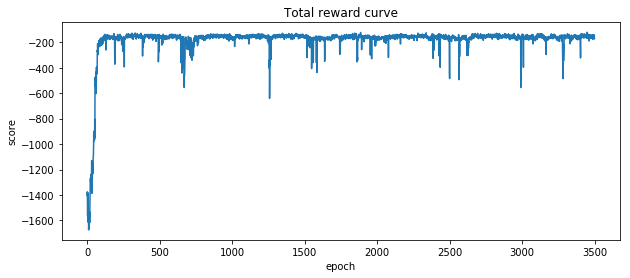
\includegraphics[width=\linewidth]{Images/ddpg-rewards.png} 
\caption{DDPG average of total reward in 100 testing}
\end{figure}

\section{DQN structure and loss}

I use two fully connected layer to build Deep Q Network as follows:

\begin{figure}[H]
\centering
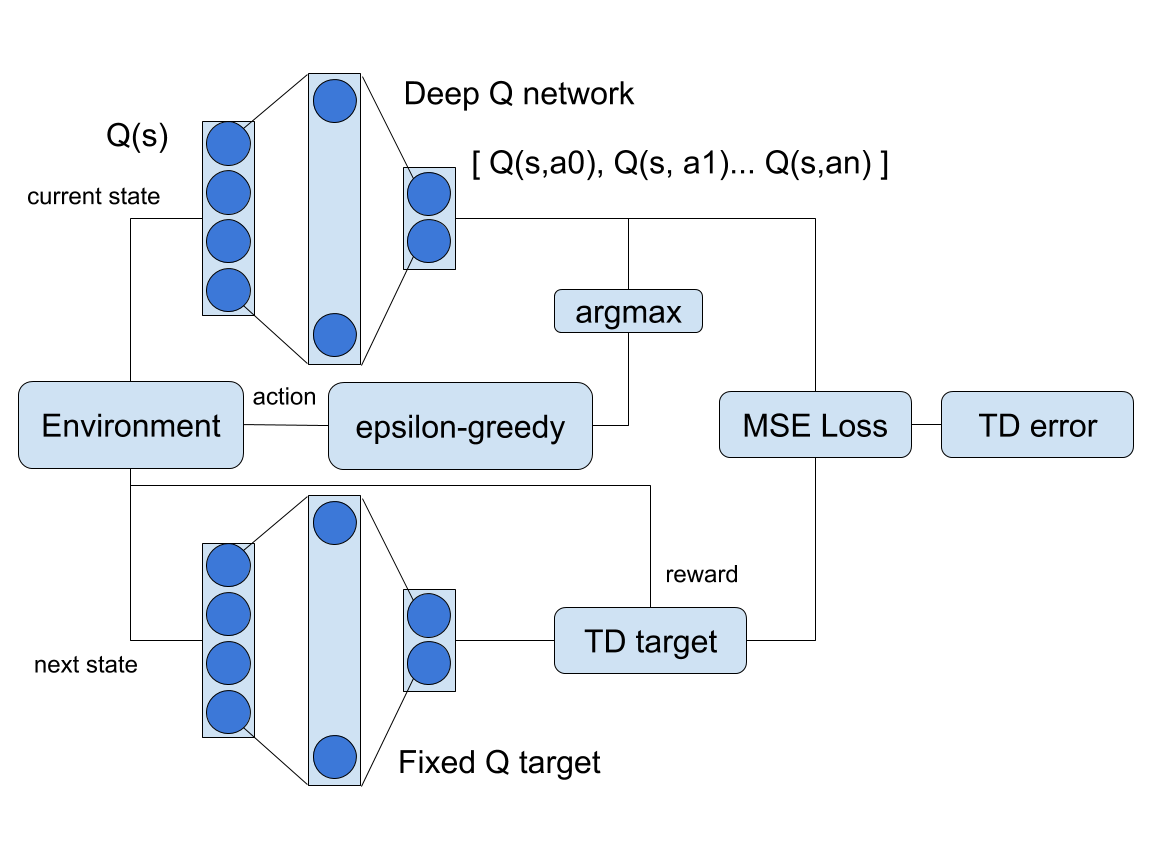
\includegraphics[width=\linewidth]{Images/dqn-arch.png} 
\caption{DQN structure and loss}
\end{figure}

The hidden size of network is 32. To avoid unstable training, use another Q network as target network to fixed target value. And implement in pytorch as follows:

\begin{minted}[frame=lines, breaklines]{python}
class DQN(nn.Module):
    def __init__(
        self, observation_space, action_space, device,
        lr=0.05, hidden_size=32, buffer_size=5000
    ):
        super(DQN, self).__init__()
        
        self.observation_space = observation_space
        if len(observation_space.shape) > 0:
            self.osize = observation_space.shape[0]
        else:
            raise NotImplementedError()
        
        self.action_space = action_space
        if len(action_space.shape) == 0:
            self.asize = action_space.n
        else:
            raise NotImplementedError()
        
        self.hidden_size = hidden_size
        
        def __DQN():
            return nn.Sequential(
                nn.Linear(self.osize, self.hidden_size),
                nn.ReLU(inplace=True),
                nn.Linear(self.hidden_size, self.asize, bias=False),
            )
        
        self.device = device
        self.eval_net = __DQN().to(self.device)
        self.target_net = __DQN().to(self.device)
        
        self.criterion = nn.MSELoss()
\end{minted}

\section{DDPG structure and loss}

DDPG has two network, one is critic and another is actor. Critic is simliar as DQN but it get action as input and only output one value. Actor uses current state to find action.

\begin{figure}[H]
\centering
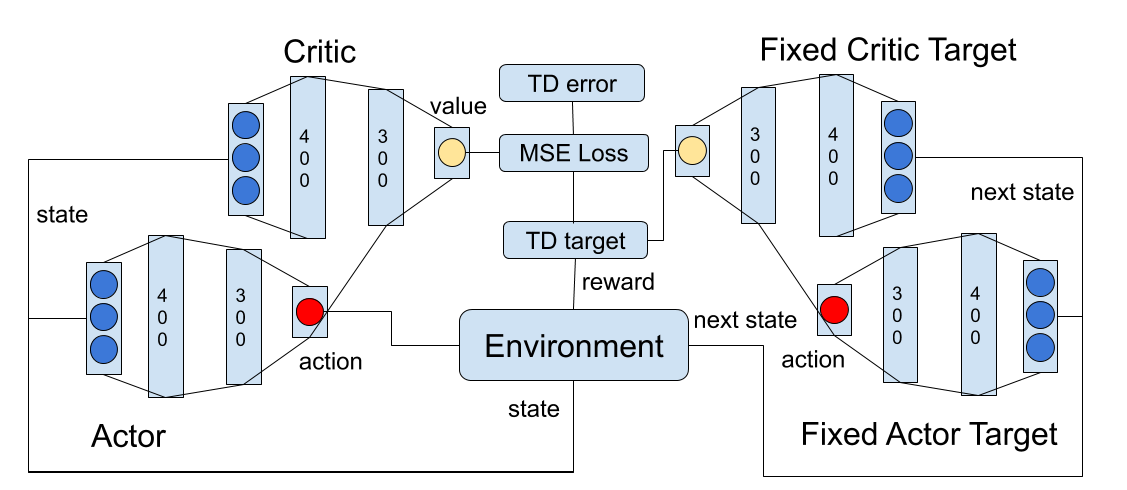
\includegraphics[width=\linewidth]{Images/ddpg-arch2.png} 
\caption{DDPG structure and loss}
\end{figure}

All layers are fully connect layer. The important point is critic need to feed action into second fully connect layer and actor need use tanh activation to control action range The whole network structure as follows:

\begin{minted}[frame=lines, breaklines]{python}
def fanin_init(size, fanin=None):
    fanin = fanin or size[0]
    v = 1. / np.sqrt(fanin)
    return torch.Tensor(size).uniform_(-v, v)

class Actor(nn.Module):
    def __init__(self, osize, asize, init_w=3e-3):
        super(Actor, self).__init__()
        
        self.osize = osize
        self.asize = asize
        
        self.main = nn.Sequential(
            nn.Linear(self.osize, 400),
            nn.ReLU(inplace=True),
            nn.Linear(400, 300),
            nn.ReLU(inplace=True),
            nn.Linear(300, self.asize),
            nn.Tanh(),
        )
        
        self.initweight(init_w)
    
    def initweight(self, init_w):
        count = 0
        for m in self.main.modules():
            if isinstance(m, nn.Linear):
                count += 1
                m.bias.data.fill_(0.0)
                if count < 3:
                    m.weight.data = fanin_init(m.weight.data.size())
                else:
                    m.weight.data.uniform_(-init_w, init_w)
    
    def forward(self, x):
        out = self.main(x)
        return out

class Critic(nn.Module):
    def __init__(self, osize, asize, init_w=3e-3):
        super(Critic, self).__init__()
        
        self.osize = osize
        self.asize = asize
        
        self.main1 = nn.Sequential(
            nn.Linear(self.osize, 400),
            nn.ReLU(inplace=True),
        )
        
        self.main2 = nn.Sequential(
            nn.Linear(400 + self.asize, 300),
            nn.ReLU(inplace=True),
            nn.Linear(300, 1),
        )
        
        self.initweight(init_w)
    
    def initweight(self, init_w):
        count = 0
        for m in list(self.main1.modules()) + list(self.main2.modules()):
            if isinstance(m, nn.Linear):
                count += 1
                m.bias.data.fill_(0.0)
                if count < 3:
                    m.weight.data = fanin_init(m.weight.data.size())
                else:
                    m.weight.data.uniform_(-init_w, init_w)
    
    def forward(self, x, a):
        out = self.main1(x)
        out = self.main2(torch.cat([out,a.reshape(-1,1)],1))
        return out

class DDPG(nn.Module):
    def __init__(
        self, observation_space, action_space
    ):
        super(DDPG, self).__init__()
    
        self.observation_space = observation_space
        self.action_space = action_space
    
        if len(observation_space.shape) > 0:
            self.osize = observation_space.shape[0]
        else:
            raise NotImplementedError()
            
        if len(action_space.shape) > 0:
            self.asize = action_space.shape[0]
        else:
            raise NotImplementedError()
        
        # u(s) -> dis of action
        self.actor = Actor(self.osize, self.asize).to(device)
        self.actor_ = Actor(self.osize, self.asize).to(device)
        self.actor_optim = torch.optim.Adam(self.actor.parameters(), lr=1e-4)
    
        # Q(s, a) -> value
        self.critic = Critic(self.osize, self.asize).to(device)
        self.critic_ = Critic(self.osize, self.asize).to(device)
        self.critic_optim = torch.optim.Adam(self.critic.parameters(), lr=1e-3)
    
        self.update()
        
        self.memory = Buffer(self.osize, self.asize, 10000)
        self.store = self.memory.store
        
        self.criterion = nn.MSELoss()
\end{minted}

\section{How to train DQN}

Deep Q Network likes Q-learning that need to estimate Q(s, a) value in lookup table. And DQN use DNN as lookup table that make DQN can handle continuous state. Therefore DQN update lookup table using back propagation as training model. I used Q target value as label or ground-truth. The equation of target value as follows:

\begin{equation}
   Q_{target} =  r_t + \gamma \max_a Q(s_{t+1}, a | \theta_Q )
\end{equation}

If $s_{t+1}$ is terminated state, then equation is only $Q_{target} = r_t$.

\subsection{Fixed target}

But update DQN frequently will make training unstable. Because DNN model not yet convergence and its value is used to next target value. To solve this problem, use fixed target model.
\par \ \par
In the begin, create two DQN model, one is target model another is evaluation model. $Q, \hat{Q}$. Convert updating equation as follows:

\begin{equation}
   Q_{target} =  r_t + \gamma \max_a \hat{Q}(s_{t+1}, a | \theta_{\hat{Q}} )
\end{equation}

Finally update target $\hat{Q}$ network through evaluation network $Q$ by every specific steps.

\subsection{Experience reply}

Because state is continuous, its space is very huge. If take whole transition in one game is too correlation and also good transition in one game is rare. Thus I store transition in buffer and take mini batch transition from buffer to train DQN.

\begin{minted}[frame=lines, breaklines]{python}
class DQN(nn.Module):
    # Omit ...

    # update target net by evaluation net
    def update(self):
        self.target_net.load_state_dict(self.eval_net.state_dict())
        
    def store_transition(self, s, a, r, s_next, done):
        transition = np.hstack((s, [a, r], s_next, done))
        # store
        self.buffer[self.buffer_count%self.buffer_size, : ] = transition
        
        self.buffer_count += 1
    
    def learn(self, batch_size, gamma=0.95):
        
        # pick data from buffer
        pick_i = np.random.choice(self.buffer_size if self.buffer_count > self.buffer_size else self.buffer_count, size=batch_size)
        x = self.buffer[pick_i, :]
        
        # clear grad
        self.eval_optimizer.zero_grad()
        
        # only use state
        q_eval, q_target = self( torch.tensor( x[:, :self.osize] ).to(self.device) , torch.tensor( x[:, -(self.osize+1):-1] ).to(self.device)) 
        
        # x[:, -1] done list
        q_target_value = torch.max(q_target, dim=1)[0].detach()
        q_target_value[np.argwhere(x[:,-1] == 1).reshape(-1)] = 0.0

        
        y = q_eval.clone().detach()
        # set y = r + \gamma max_a( Q_target(s', a) )
        y[np.arange(batch_size), x[:, self.osize]]  = torch.tensor(x[:, self.osize+1]).float() + (gamma * q_target_value)
        
        # get loss
        loss = self.criterion(q_eval, y)
        
        # update weight
        loss.backward()
        
        # prevent too huge grad
        #for param in self.eval_net.parameters():
        #    param.grad.data.clamp_(-1, 1)
        
        self.eval_optimizer.step()
        
        return loss
\end{minted}

\section{How to implement epsilon-greedy action}

If always use action result from model, model can't explore new space in environment. To avoid this problem, model sometimes random a action.

\begin{minted}[frame=lines, breaklines]{python}
epsilon_thr = epsilon_end + ( (epsilon_start - epsilon_end) * np.exp(-1. * epoch / epsilon_decay) )

# choose action
if np.random.rand() < epsilon_thr:
    action = np.random.randint(agent.asize)
else:
    action = agent.think(observation)
\end{minted}

I decrease epsilon threshold along with epoch increasing.

\section{Critic and Actor updating in DDPG}

DDPG also use fixed target and experience reply to train model. I initial actor as $u(s|\theta_u)$ and $\hat{u}(s | \theta_{\hat{u}})$ and critic as $Q(s, a | \theta_Q)$ and $\hat{Q}(s, a|\theta_{\hat{Q}})$. Critic likes DQN, it need to estimate value. Thus update it with equation as follows:

\begin{equation}
    Q_{target} = r_t + \gamma \hat{Q}(s_{t+1}, \hat{u}(s_{t+1}|\theta_{\hat{u}}) | \theta_{\hat{Q}})
\end{equation}

Loss can use mean square error as follows:

\begin{equation}
    L = \frac{1}{N} \sum (Q_{target} - Q(s_t, a_t | \theta_Q))^2
\end{equation}

Using previous equation let critic can know how many reward in specific state and action. Because of it, actor depend on critic to know which action to generate better reward. 

\subsection{How to calculate the actor's gradients}

Actor's objective is making better reward in continuous action space. I use equation as follows to reach it.

\begin{equation}
    L = - Q(s, u(s | \theta_u) | \theta_Q)
\end{equation}

I minimize loss like maximize reward from actor's action.
\par \ \par
Use chain rule to show how to calculate gardient.

\begin{equation}
    L =  - Q(s, a | \theta_Q), \  a = u(s | \theta_u)
\end{equation}
\begin{align}
    \frac{\nabla L }{ \nabla \theta_u } & = - \frac{ \nabla Q(s, a | \theta_Q) }{ \nabla a } \frac{\nabla a}{\nabla u(s | \theta_u)} \frac{\nabla u(s | \theta_u)}{\nabla \theta_u} \\
    & = - \frac{ \nabla Q(s, a | \theta_Q) }{ \nabla u(s | \theta_u) }\frac{\nabla u(s | \theta_u)}{\nabla \theta_u}
\end{align}


\begin{minted}[frame=lines, breaklines]{python}
class DDPG(nn.Module):
    # Omit ...
    def update(self, tau=None):
        if tau is None:
            self.actor_.load_state_dict(self.actor.state_dict())
            self.critic_.load_state_dict(self.critic.state_dict())
        else:
            soft_update(self.actor_, self.actor, tau)
            soft_update(self.critic_, self.critic, tau)
            
    def learn(self, batch_size, gamma=0.99):
        s, a, r, s_, done = self.memory.miniBatch(batch_size)

        with torch.no_grad():
            q_ = self.critic_(
                to_tensor(s_), 
                self.actor_(to_tensor(s_)) 
            )
        
        q_target = to_tensor(r) + ( gamma * to_tensor(1.0 - done.astype(np.float))*q_ )
        q_target = q_target.detach()
        
        # Critic learn
        self.critic_optim.zero_grad()
        
        #s = to_tensor(s)
        q = self.critic(
            to_tensor(s),
            to_tensor(a)
        )
        loss_value = self.criterion(q, q_target)
        loss_value.backward()
        
        self.critic_optim.step()
        
        # Actor learn
        self.actor_optim.zero_grad()
        
        loss_policy = -self.critic(
            to_tensor(s),
            self.actor(to_tensor(s))
        )
        
        loss_policy = loss_policy.mean()
        loss_policy.backward()
        
        self.actor_optim.step()
        
        self.update(tau=1e-3)
        
        return loss_value, loss_policy
\end{minted}

Finally, I need to update target with $\tau$.

\begin{align}
    \theta_{\hat{Q}} = (1 - \tau) \theta_{\hat{Q}} + \tau \theta_Q
    \theta_{\hat{u}} = (1 - \tau) \theta_{\hat{u}} + \tau \theta_u
\end{align}

\begin{minted}[frame=lines, breaklines]{python}
def soft_update(target, source, tau):
    for target_param, param in zip(target.parameters(), source.parameters()):
        target_param.data.copy_(
            target_param.data * (1.0 - tau) + param.data * tau
        )
\end{minted}

\section{Code explanation}

First, create environment. I wrap open AI gym can show in jupyter notebook.

\begin{minted}[frame=lines, breaklines]{python}
def myrender(self, title=''):
    plt.title(title)
    plt.imshow(self.old_render(mode='rgb_array'))
    plt.axis('off')
    plt.show()
    clear_output(wait=True)
    time.sleep(1/30)
    
def wrapper_gymenv(env):
    env = NormalizedAction(env) # only need in DDPG
    env.old_render = env.render
    env.render = lambda title='': myrender(env, title)
    return env

env = gym.make('Pendulum-v0') 
# or env = gym.make('CartPole-v0')
env = wrapper_gymenv(env)
\end{minted}

Second, create agent.

\begin{minted}[frame=lines, breaklines]{python}
agent = DDPG(env.observation_space, env.action_space) 
# or agent = DQN(env.observation_space, env.action_space, torch.device("cpu"))

\end{minted}

Third, training agent with environment. In DQN, I need to store best agent in training.

\begin{minted}[frame=lines, breaklines]{python}
train(agent, 3500, 64) 
# best_agent = train(agent, 1000, 128, 50) in DQN
\end{minted}

Train procedures are very similar between DQN and DDPG. I use DDPG training as example. In every epoch, I reset environment and send action to environment through agent or random action. (In DQN, use epsilon-greedy action) When environment responses next state and reward, I store state, action , reward, next state and done (Is game end ?) into experience buffer. If buffer has enough transition, I let agent learn from experience buffer with mini batch size. (In DDPG case, it is 64) If environment reach terminated state, I evaluation agent to get average total rewards. After that I store some metric and show result. 

\begin{minted}[frame=lines, breaklines]{python}
def train(
    agent, epoch_size, batch_size
):
    
    for epoch in range(len(agent.metrics), epoch_size):
        # play
        
        observation = env.reset()
        score = 0.0
        step = 0
        
        loss_v_t = []
        loss_p_t = []
        
        agent.train()
        agent.reset()
        
        while True:
            
            if agent.memory.buffer_count <= 100:
                action = agent.random_think()
            else:
                action = agent.think(observation, True)
                
            # do action
            observation_next, reward, done, info = env.step(action)
            step += 1
            
            agent.store(observation, action, reward, observation_next, done)
            
            if agent.memory.buffer_count > 100:
                loss_value, loss_policy = agent.learn(batch_size)
                loss_v_t.append(loss_value.item())
                loss_p_t.append(loss_policy.item())
            
            # update state
            observation = observation_next
            
            if done:
                break
        
        test_score = np.mean([play(agent, show=False) for _ in range(100)])
        
        # metrics
        loss_v_t = np.average(loss_v_t) if len(loss_v_t) > 0 else 0.0
        loss_p_t = np.average(loss_p_t) if len(loss_p_t) > 0 else 0.0
            
        agent.metrics.append( (test_score, loss_v_t, loss_p_t) )
        
        clear_output(wait=True)
        print('#{:6.0f}: score : {:5.4f}'.format(epoch, test_score))
\end{minted}

Fourth, evaluation agent without any random.

\begin{minted}[frame=lines, breaklines]{python}
def evaluation(
    agent, eval_size
):
    scores = []
    for i in range(eval_size):
        scores.append( play(agent, show=False) )
    
    print('mean = {}, max = {}'.format(np.mean(scores), np.max(scores)))
    
    return scores

scores = evaluation(agent, 1000)
\end{minted}

\section{CartPole with DQN performance}

\par
\begin{table}[H]
    \centering
    \csvautobooktabular{dqn.csv}
    \caption{CartPole with DQN performance}
    %\label{tab:my_label}
\end{table}

\section{Pendulum with DDPG performance}

\par
\begin{table}[H]
    \centering
    \csvautobooktabular{ddpg.csv}
    \caption{Pendulum with DDPG performance}
    %\label{tab:my_label}
\end{table}

\begin{figure}[H]
\centering
% \includegraphics[width=\linewidth]{path/to/image}
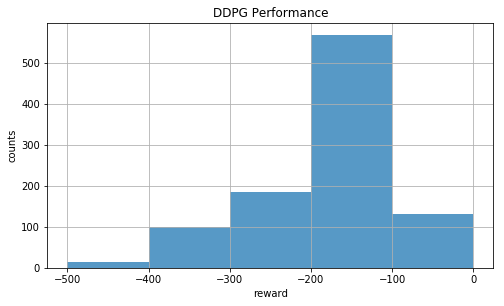
\includegraphics[width=\linewidth]{Images/ddpg-performance.png}
\caption{DDPG rewards distribution}
\end{figure}

% -----------------------------

% \section{Discussion}

% --------------------------------------------------------------
%     You don't have to mess with anything below this line.
% --------------------------------------------------------------
 
\end{document}